%!TEX root = ../thesis.tex

\cleardoublepage
\chapter{Introduction}
\label{cha:introduction}

%%=========================================
\section{Motivation and Problem Description}
\label{sec:motivation}

One of the aims for the fifth generation of mobile networks (5G) and it's successors will be a greater diversification of the classes of service. As the use cases for these networks evolve, there is a greater need for quality of service (QoS) tailored to each use case. For example, in Industrial Internet of Things (IIoT) applications the bandwidth requirements are often quite low, however the requirements on latency, jitter, and reliability may be extremely stringent. Supporting these kinds of classes of service can be  a challenge for mobile network operators (MNOs) and will require novel approaches to familiar problems, such as backhaul.

With more backhaul solutions becoming available (i.e. LEO satellite links, and mmWave backhaul) and adding to the existing set of options (DSL, optical fibre, DOCSIS, etc.) network operators may choose to utilize more than one backhaul connection at once in order to increase the available bandwidth or to utilize the different qualities of the backhaul links. Such a situation, could then be used to achieve higher quality of service by intelligently selecting on which link to forward packets. This approach bears similarity to multihoming as well as to multi-path routing, and can take inspiration from the existing body of research in these fields which has demonstrated that QoS can be improved by using multiple paths simultaneously \cite{akella_measurement-based_nodate, shu_tao_improving_2005, habib_improving_2007, goldenberg_optimizing_nodate}.


%\LTXtable{\textwidth}{tab/scenario1_sensor}

%%=========================================
\section{Goal of the Thesis}
\label{sec:goal}

\begin{figure}[h]
    \centering
        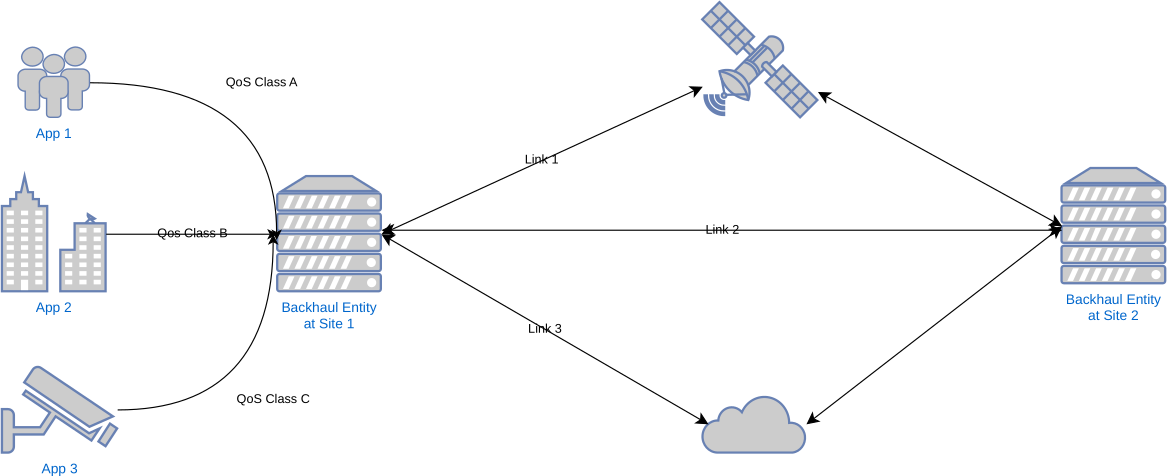
\includegraphics[width=\textwidth]{fig/use_cases.png}
        \caption{Use Case for the Backhaul Entity}
        \label{fig:use}
\end{figure}


\begin{figure}[h]
    \centering
        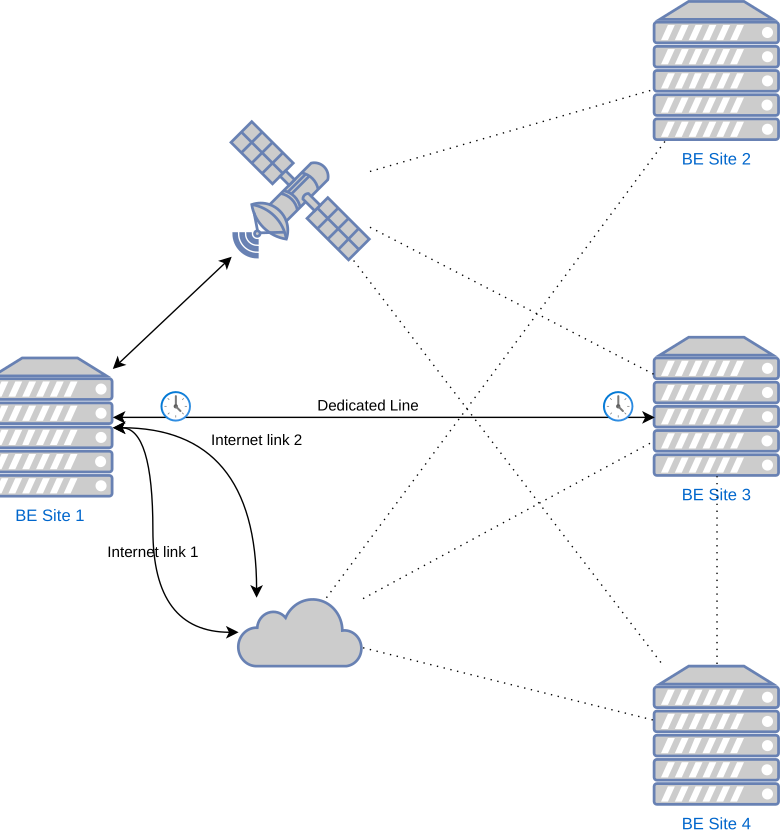
\includegraphics[width=0.75\textwidth, height=0.75\textwidth]{fig/mesh_network.png}
        \caption{Network Design of Interconnected Backhaul Sites}
        \label{fig:mesh}
\end{figure}

The goal of this thesis is to design a backhaul entity, that can be placed at the ingress and egress point of connected networks, and which can intelligently forward packets on one or more links in order to meet specific QoS requirements. The performance of this approach will then be quantitatively analysed in experiments. Looking at figure \ref{fig:use} we can see how this is envisioned to work: A backhaul entity is deployed in 2 or more sites which have more than one egress link. Then, using the multiple links, the traffic is backhauled to the second site, while respecting it's QoS requirements. An example of how this entity could be deployed in multiple sites, interconnected in a mesh network, can be seen in figure \ref{fig:mesh}. This could allow network operators to provide more reliable quality of service for it's users, especially for important applications (e.g. between an industrial controlling site, and multiple factories).

%%=========================================
\section{Structure of the Thesis}
\label{sec:structure}

The thesis will be structured as follows:

\begin{enumerate}
\item{\textit{Design}: Research existing approaches and solutions, and design an approach for reliable backhaul over multiple paths/links}
\item{\textit{Implementation}: Implement said approach in a basic testbed consisting of a traffic generator, various link emulators, measurement devices, and the backhaul entities}
\item{\textit{Evaluation}: Analyse the performance of the backhaul entity according to its ability to reduce latency, improve jitter, and provide any other QoS requirements. And compare it's performance with the performance of each individual link, as well as the performance of a round robin packet forwarding approach which utilises each link equally.}

\end{enumerate}

\begin{figure}[h]
    \centering
        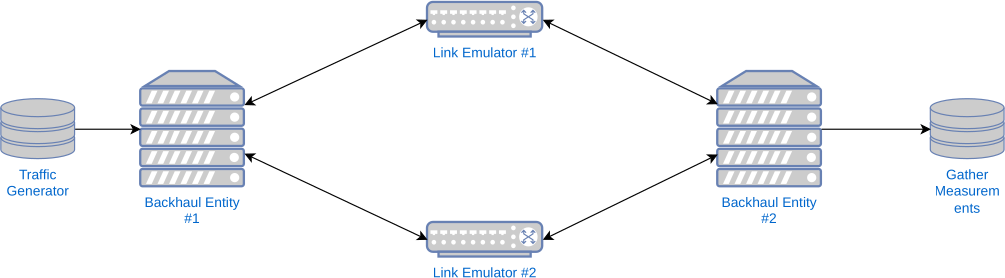
\includegraphics[width=\textwidth]{fig/testbed.png}
        \caption{Testbed Setup}
        \label{fig:testbed}
\end{figure}


\section{Envisioned Approach}

\subsection{Collecting Per-Link Metrics}
In order to realize such a backhaul entity, the entity needs to be able to maintain a  set of metrics about the available links to aid it in choosing which link or links to utilize. This may not always be straightforward, and could require prediction of link quality based on previous measurements. Beyond this, the entity also needs a method through which the QoS it needs to provide for a given flow can be externally configured. Only then can the actual approach be implemented.

\subsection{How to Guarantee QoS}

The design of this approach is also an interesting challenge. One idea to improve jitter when backhauling across multiple links is to duplicate packets and forward them both across different links, and have the backhaul entity on the other end buffer incoming packets and release them at a constant rate. This way in the event of a packet being lost on one link, the other link is still able to receive it and the delay caused by retransmission is avoided. For reducing latency it would appear likely that the simplest approach may be a greedy method which always selects the lowest latency connection. However there is room for nuance here since the connection must not be overloaded and also because certain traffic may have very relaxed latency requirements but use up more bandwidth. This means monitoring the load on any one link will be important. Finally there are also more intelligent approaches, i.e. integer linear programming which could be used to optimally satisfy certain requirements.

As can be seen from this short overview, there are a littany of factors to consider and approaches which could be taken. It will be important to maintain a strict focus in this thesis and not try to optimize too many requirements at once, or try to consider too many different metrics for any given link. The number of QoS factors which will be taken into consideration and adjusted for must be kept small, in addition to this, the number of link metrics which will be analysed must also be kept to a reasonable amount.

\subsection{Approaches in existing literature}

TODO (ILP approach from some paper..., QoS thing which uses past performance and adjusts the window for how long to use a connection)

\section{Scope and Potential Extensions}

It may be worth investigating the effect of using information theoretical approaches such as network coding, or forward error correction. These methods can, respectively, improve throughput and provide protection against packet loss. However it is not clear if it would be feasible to integrate them into the backhaul entity's packet scheduling algorithm, and how much effort that may require.

One other potential extension of this thesis would be to compare performance against an offline scheduler which knows the traffic patterns and link patterns in advance. This could provide a baseline for what could be considered optimal performance. However to design such a scheduler and train it offline before the online tests could be unrealistic for the scope of this thesis.

At the very least both of these points bear mentioning in the future work section.